% Stack diagram for the "Where {anvl} sits" slide.
% Styled to match three-transformations.tex: rounded boxes, Stealth arrows,
% and the same blue highlight for the parts that are ours / the shared core.
\documentclass[tikz, border=8pt]{standalone}
\usetikzlibrary{arrows.meta, positioning, fit, backgrounds}

\begin{document}
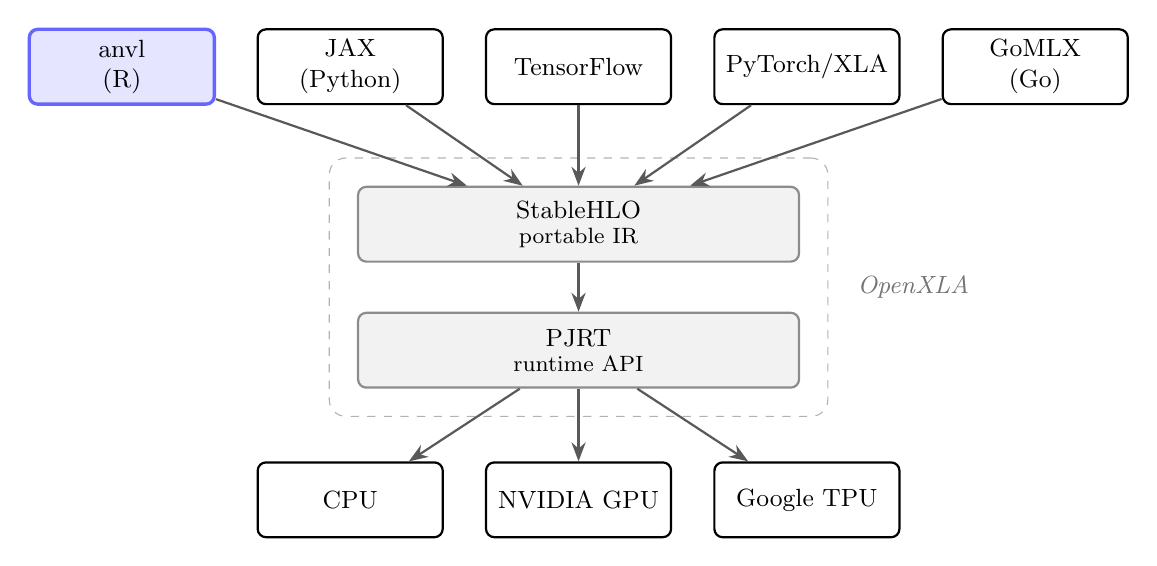
\begin{tikzpicture}[
  every node/.style={font=\small},
  box/.style={
    draw, rounded corners=3pt, thick,
    minimum width=2.35cm, minimum height=0.95cm, align=center
  },
  ours/.style={box, fill=blue!10, draw=blue!60, very thick},
  % The core is deliberately NOT the same blue as anvl: blue marks what is
  % ours, grey the shared stack we did not build.
  core/.style={box, fill=black!5, draw=black!45, minimum width=5.6cm},
  arr/.style={-{Stealth[length=2.4mm, width=1.8mm]}, thick, draw=black!65}
]
  % --- frontends -----------------------------------------------------------
  \node[ours] (anvl) at (0,    3.9) {anvl\\(R)};
  \node[box]  (jax)  at (2.9,  3.9) {JAX\\(Python)};
  \node[box]  (tf)   at (5.8,  3.9) {TensorFlow};
  \node[box]  (pt)   at (8.7,  3.9) {PyTorch/XLA};
  \node[box]  (go)   at (11.6, 3.9) {GoMLX\\(Go)};

  % --- the shared core -----------------------------------------------------
  \node[core] (shlo) at (5.8, 1.9) {StableHLO\\[-2pt]{\footnotesize portable IR}};
  \node[core] (pjrt) at (5.8, 0.3) {PJRT\\[-2pt]{\footnotesize runtime API}};
  \draw[arr] (shlo) -- (pjrt);

  % --- devices -------------------------------------------------------------
  \node[box] (cpu) at (2.9,  -1.6) {CPU};
  \node[box] (gpu) at (5.8,  -1.6) {NVIDIA GPU};
  \node[box] (tpu) at (8.7,  -1.6) {Google TPU};

  \foreach \f in {anvl,jax,tf,pt,go} \draw[arr] (\f) -- (shlo);
  \foreach \d in {cpu,gpu,tpu}       \draw[arr] (pjrt) -- (\d);

  \begin{scope}[on background layer]
    \node[draw=black!30, dashed, rounded corners=6pt, inner sep=10pt,
          fit=(shlo)(pjrt)] (xla) {};
  \end{scope}
  \node[anchor=west, font=\small\itshape, text=black!55]
        at ([xshift=7pt]xla.east) {OpenXLA};
\end{tikzpicture}
\end{document}
